\documentclass[american,titlepage]{ntnuthesis}

% --- Ams theorem definitions --- %
    \usepackage{amsthm}

    % --- Defining theorem env --- % 
    \theoremstyle{plain}
    \newtheorem{thm}{Theorem}[section]
    \newtheorem{lemma}[thm]{Lemma}
    \newtheorem{prop}[thm]{Proposition}
    \newtheorem{cor}{Corollary}[thm]

    % --- Defining definition env --- %
    \theoremstyle{definition}
    \newtheorem{definition}[thm]{Definition}

    % --- Defining remark env --- %
    \theoremstyle{remark}
    \newtheorem{remark}[thm]{Remark}
    \newtheorem{construction}[thm]{Construction}
    \newtheorem{observation}[thm]{Observation}

    % --- Defining proof environment --- %

% --- Front page --- %
    \title{Sha-Categories \& Quasi-isomorphisms}
    \shorttitle{Sha Cat}
    \author{Thomas Wilskow Thorbjørnsen}
    \shortauthor{Thorbjørnsen}
    \date{\today}

% --- Bibliography --- %
    \addbibresource{thesis.bib}

% --- Glossary --- %
    
% From https://www.overleaf.com/learn/latex/Glossaries

\makeglossaries % Prepare for adding glossary entries


\newglossaryentry{latex}
{
        name=latex,
        description={Is a mark up language specially suited for
scientific documents}
}

\newglossaryentry{bibliography}
{
        name=bibliography,
        plural=bibliographies,
        description={A list of the books referred to in a scholarly work,
typically printed as an appendix}
}

\newglossaryentry{maths}
{
    name=mathematics,
    description={Mathematics is what mathematicians do}
}


% --------------------
% ----- Acronyms -----
% --------------------

\newacronym{phd}{PhD}{philosophiae doctor}
\newacronym{CoPCSE}{CoPCSE@NTNU}{Community of Practice in Computer ScienceEducation at NTNU}
\newacronym{gcd}{GCD}{Greatest Common Divisor}
 % add glossary and acronym lists before document

% --- Folder structure --- %
    \usepackage{subfiles} 
    % Allows compilation of each subfile, rather to compile everything at once
    % Subfiles must have this file as option while using the documentclass subfile
    % Loading a subfile is done with \subfile{"path-to-file"}

\begin{document}

    % --- Preface --- %
    \subfile{chapters/preface/preface.tex}

    % --- Structure --- %
    \tableofcontents % This lists each listable section, subsection and subsubsection 
    % \listoffigures % This lists each figure
    % \listoftables % This lists each table
    % \lstlistoflistings % This lists each code snippet

    \printglossary[type=\acronymtype] % Print acronyms
    \printglossary                    % Print glossary

    % --- Chapter 1 --- %
    \chapter{Preliminaries}

        \subfile{chapters/preliminaries/localization/localization.tex}
        \newpage

        \subfile{chapters/preliminaries/triangulated/triangulated.tex}

    \chapter*{\bibname}
    \printbibliography[heading=none]

    % % First paper

\begin{paper}{papers/landes1951scrutiny.pdf}{paper:scrutiny}
    Here, you may add a description of the paper, an illustration, or just give the bibliographic reference:
    \begin{quote}
        \fullcite{landes1951scrutiny}
    \end{quote}
    Or you may leave it empty, if you like.
\end{paper}

% Second paper etc.

    \appendix
% \chapter{Additional Material}
\label{app:additional}

Additional material that does not fit in the main thesis but may still be relevant to share, e.g., raw data from experiments and surveys, code listings, additional plots, pre-project reports, project agreements, contracts, logs etc., can be put in appendices. Simply issue the command \texttt{\textbackslash appendix} in the main \texttt{.tex} file, and make one chapter per appendix.

If the appendix is in the form of a ready-made PDF file, it should be supported by a small descriptive text, and included using the \texttt{pdfpages} package. To illustrate how it works, a standard project agreement (for the IE faculty at NTNU in Gjøvik) is attached here. You would probably want the included PDF file to begin on an odd (right hand) page, which is achieved by using the \texttt{\textbackslash cleardoublepage} command immediately before the \texttt{\textbackslash includepdf[]\{\}} command. Use the option \texttt{[pages=-]} to include all pages of the PDF document, or, e.g., \texttt{[pages=2-4]} to include only the given page range.

\cleardoublepage
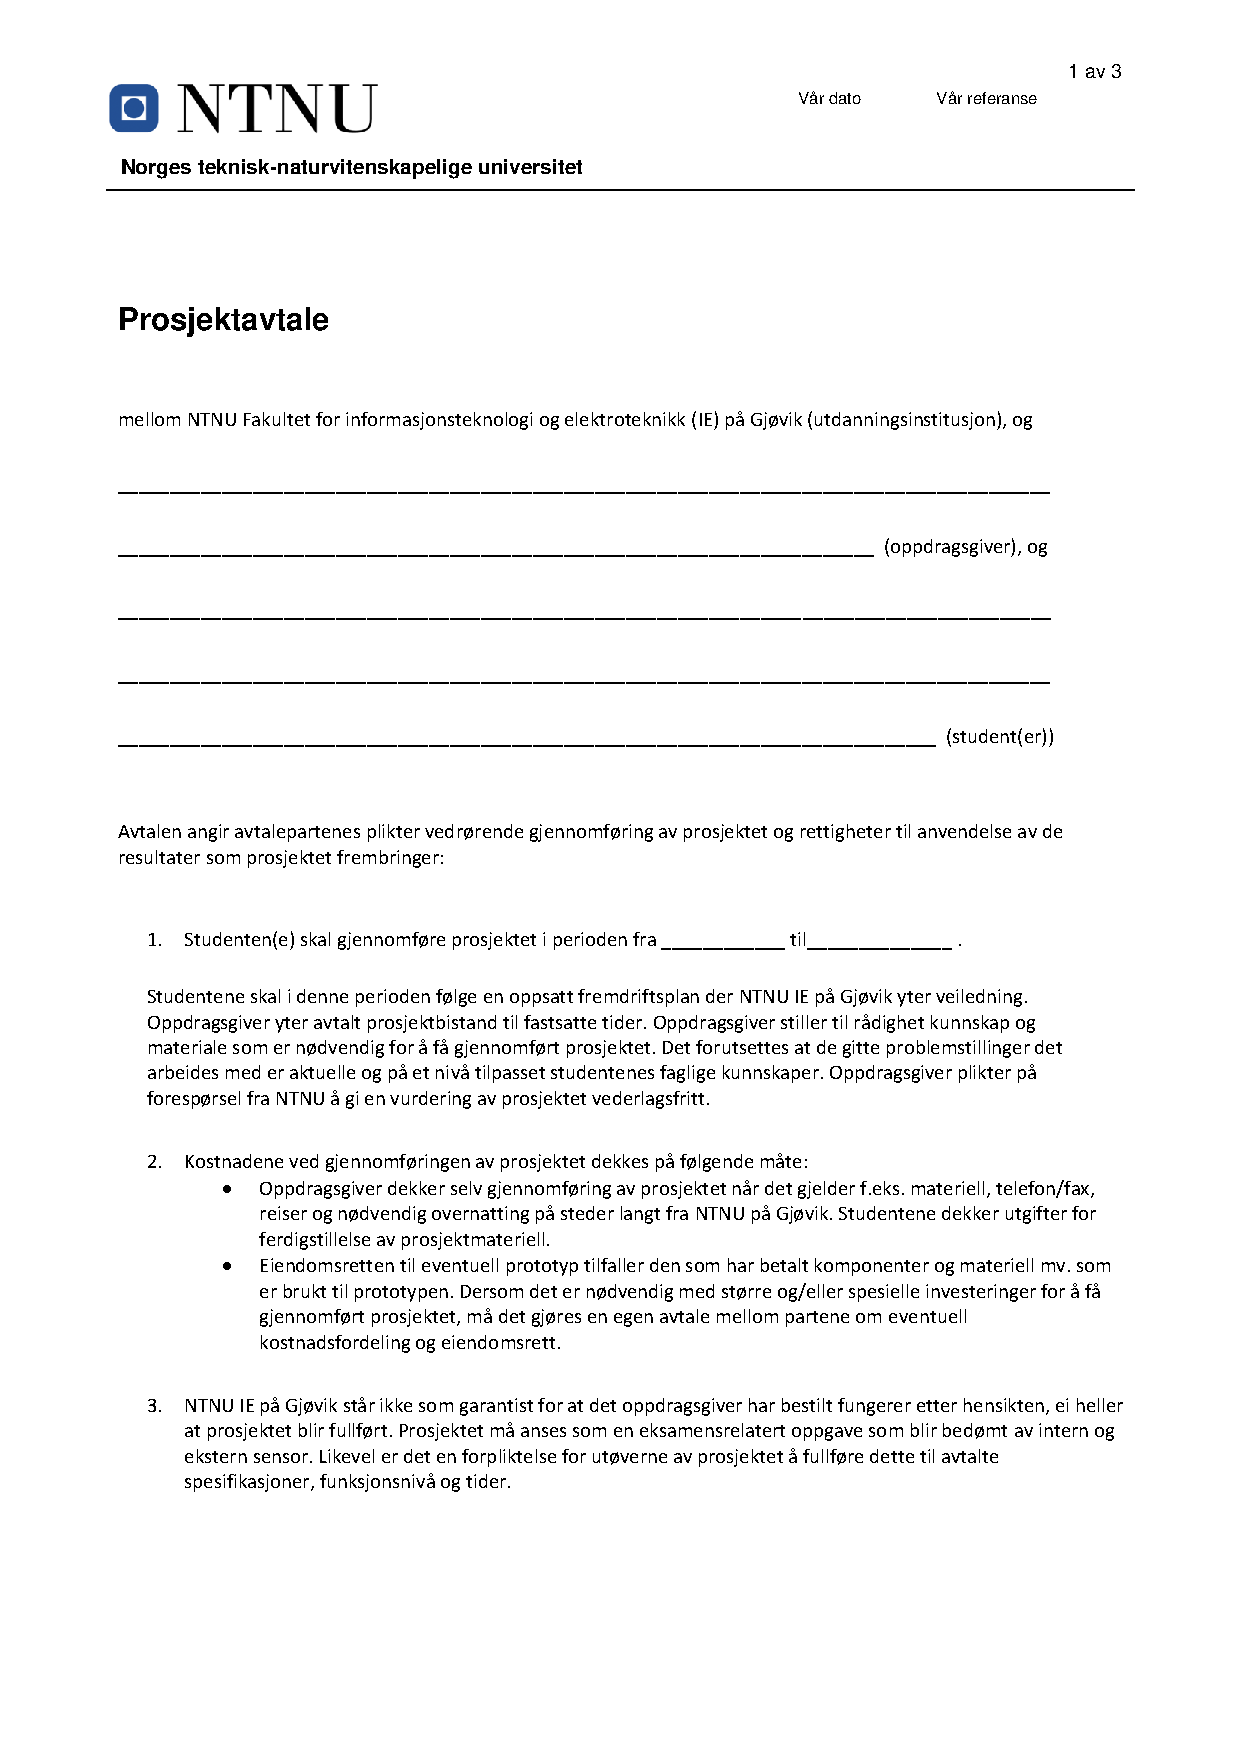
\includepdf[pages=-]{appendices/NTNUProsjektavtale.pdf}

\end{document}
